% !TEX root = Projektdokumentation.tex
\section{Anhang}
\subsection{Detaillierte Zeitplanung}
\label{app:Zeitplanung}
\tabelleAnhang{ZeitplanungKomplett}
\clearpage

\subsection{Ressourcen}
\label{app:Ressourcen}
Hardware
\begin{itemize}
    \item Büroarbeitsplatz mit MS Windows Desktop-PC
\end{itemize}
Software
\begin{itemize}
    \item Microsoft Windows 10 Pro -- Betriebssystem
    \item Microsoft Visual Studio Enterprise 2022 (64-bit) -- v17.3.6 -- Entwicklungsumgebung
    \item JetBrains ReSharper Tools v2022.1 -- Erweiterung für Visual Studio für \ua Refactoring
    \item Microsoft Visual Studio Code v1.72.1 -- Texteditor mit Highlightfunktion und vielen Erweiterungen
    \item draw.io -- Programm zum Erstellen von UML-Diagrammen
    \item syntevo SmartGit v21.1.1 -- Clientprogramm zur Versionsverwaltung mit Git
    \item GitLab -- intern gehostete Versionsverwaltung
    \item Progress Telerik UI -- Framework für Benutzeroberflächen
    \item Google Chrome (64-bit) v105.0.5195.102 -- Webbrowser
    \item MiKTeX -- Distribution des LaTeX-Textsatzsystems
    \item LaTeX Workshop -- Erweiterung für Visual Studio Code zum Editiren von LaTeX-Dokumenten
    \item Postman -- Tool zur Abfrage von Web-\acs{API}s
    \item Screenpresso -- Tool zum Erstellen von Screenshots
\end{itemize}
Personal
\begin{itemize}
    \item Umschüler Fachinformatiker für Anwendungsentwicklung -- Umsetzung des Projekts
    \item Entwickler der Softwareabteilung  -- Code-Review, technische Abnahme, Deployment
    \item Entwicklerin der Fachabteilung -- Anforderungen des ReklaTool, Unterstützung beim Entwurf der Benutzeroberfläche,
    Endabnahme der Anwendung
\end{itemize}
\clearpage

\subsection{Break-Even-Point}
\label{app:BreakEvenPoint}
\begin{figure}[!htb]
    \centering
    \includegraphicsKeepAspectRatio{BreakEvenPoint.png}{1}
    \caption{Break-Even-Point}
\end{figure}

\subsection{Lastenheft (Auszug)}
\label{app:Lastenheft}
Es folgt ein Auszug aus dem Lastenheft mit Fokus auf die Anforderungen:

Die Anwendung muss folgende Anforderungen erfüllen: 
\begin{enumerate}[itemsep=0em,partopsep=0em,parsep=0em,topsep=0em]
\item Verarbeitung der Moduldaten
	\begin{enumerate}
	\item Die Anwendung muss die von Subversion und einem externen Programm bereitgestellten Informationen (z.B. Source-Benutzer, -Datum, Hash) verarbeiten.
	\item Auslesen der Beschreibung und der Stichwörter aus dem Sourcecode.
	\end{enumerate}
\item Darstellung der Daten
	\begin{enumerate}
	\item Die Anwendung muss eine Liste aller Module erzeugen inkl. Source-Benutzer und -Datum, letztem Commit-Benutzer und -Datum für alle drei Umgebungen. 
	\item Verknüpfen der Module mit externen Tools wie z.B. Wiki-Einträgen zu den Modulen oder dem Sourcecode in Subversion.
	\item Die Sourcen der Umgebungen müssen verglichen und eine schnelle Übersicht zur Einhaltung des allgemeinen Entwicklungsprozesses gegeben werden. 
	\item Dieser Vergleich muss auf die von einem bestimmten Benutzer bearbeiteten Module eingeschränkt werden können. 
	\item Die Anwendung muss in dieser Liste auch Module anzeigen, die nach einer Bearbeitung durch den gesuchten Benutzer durch jemand anderen bearbeitet wurden. 
	\item Abweichungen sollen kenntlich gemacht werden. 
	\item Anzeigen einer Übersichtsseite für ein Modul mit allen relevanten Informationen zu diesem.
	\end{enumerate}
\item Sonstige Anforderungen
	\begin{enumerate}
	\item Die Anwendung muss ohne das Installieren einer zusätzlichen Software über einen Webbrowser im Intranet erreichbar sein.
	\item Die Daten der Anwendung müssen jede Nacht \bzw nach jedem \acs{SVN}-Commit automatisch aktualisiert werden. 
	\item Es muss ermittelt werden, ob Änderungen auf der Produktionsumgebung vorgenommen wurden, die nicht von einer anderen Umgebung kopiert wurden. Diese Modulliste soll als Mahnung per E-Mail an alle Entwickler geschickt werden (Peer Pressure).
	\item Die Anwendung soll jederzeit erreichbar sein.
	\item Da sich die Entwickler auf die Anwendung verlassen, muss diese korrekte Daten liefern und darf keinen Interpretationsspielraum lassen.
	\item Die Anwendung muss so flexibel sein, dass sie bei Änderungen im Entwicklungsprozess einfach angepasst werden kann.
	\end{enumerate}
\end{enumerate}


\clearpage

\subsection{Aktivitätsdiagramm}
\label{app:Aktivitaet}
\begin{figure}[!htb]
    \centering
    \includegraphicsKeepAspectRatio{Aktivitaetsdiagramm.png}{1}
    \caption{Aktivitätsdiagramm}
\end{figure}
\clearpage

\subsection{Use-Case-Diagramm}
\label{app:UseCase}
\begin{figure}[!htb]
    \centering
    \includegraphicsKeepAspectRatio{UseCaseDiagram.png}{1}
    \caption{Use-Case-Diagramm}
\end{figure}
\clearpage

\subsection{Systemkontextdiagramm}
\label{app:Systemkontext}
\begin{figure}[!h]
    \centering
    \includegraphicsKeepAspectRatio{Systemkontext.png}{0.9}
    \caption{Systemkontextdiagramm}
\end{figure}

\subsection{MVC-Entwurfsmuster}
\label{app:MVC}
\begin{figure}[!h]
    \centering
    \includegraphicsKeepAspectRatio{MVC.png}{0.9}
    \caption{MVC-Entwurfsmuster}
\end{figure}
\clearpage

\thispagestyle{empty}
\includepdf[fitpaper=true,pages=2,addtolist={2,figure,Sequenzdiagramm,app:Sequenzdiagramm},
addtotoc={2,subsection,1,Sequenzdiagramm,app:Sequenzdiagramm}]{Bilder/Anhang_A3.pdf}
\clearpage

\setcounter{subsection}{9}
\subsection{Pflichtenheft (Auszug)}
\label{app:Pflichtenheft}

\subsubsection*{Zielbestimmung}
\begin{enumerate}
    \item Plattform
        \begin{enumerate}
            \item Die Anwendung wird in \Fachbegriff{C\# 10.0} umgesetzt.
            \item Das benutzte Framework ist \Fachbegriff{.NET 6.0}.
            \item Als Webframework wird \Fachbegriff{ASP.Net Core MVC} genutzt.
            \item Die Webanwendung läuft im Intranet der \acs{Icam}.
            \item Die Versionskontrolle erfolgt über \Fachbegriff{Git}.
        \end{enumerate}
    \item Benutzeroberfläche
        \begin{enumerate}
            \item Die Benutzeroberfläche wird mit Komponenten von \Fachbegriff{TelerikUI} umgesetzt.
            \item Zur Erstellung werden die Programmiersprachen \Fachbegriff{C\#} und \acs{JS} verwendet.
            \item Als Auszeichnungssprachen werden \acs{HTML} und \acs{CSS} benutzt.
            \item Die Benutzeroberfläche wird für die Betrachtung auf einem Desktop-PC entworfen.
            \item Daten werden in Tabellen strukturiert.
            \item Teilbereiche sollen über Reiter erreichbar sein.
            \item Die Suchfunktion soll einschränkbar sein.
        \end{enumerate}
    \item Geschäftslogik
        \begin{enumerate}
            \item Die Einbindung von \Fachbegriff{Services} erfolgt übe \acs{DI}.
            \item Aus der \acs{API}-Antwort heraus wird eine \acs{XML}-Datei zum Download bereitgestellt.
            \item Aus der \acs{API}-Antwort heraus wird eine \acs{PDF}-Datei zum Download bereitgestellt.
            \item Suchergebnisse werden in einem \Fachbegriff{Cache} zwischengespeichert.
        \end{enumerate}
\end{enumerate}
\clearpage

\thispagestyle{empty}
\includepdf[fitpaper=true,pages=3,addtolist={3,figure,Klassendiagramm,app:Klassendiagramm},
addtotoc={3,subsection,1,Klassendiagramm,app:Klassendiagramm}]{Bilder/Anhang_A3.pdf}

\setcounter{subsection}{11}
\subsection{Datenmodell}
\label{app:Datenmodell}
\begin{figure}[h]
    \centering
    \includegraphicsKeepAspectRatio{XML_Antwort.png}{0.5}
    \caption{XML-Modell für Antwort}        
\end{figure}
\begin{figure}[!htb]
    \centering
    \includegraphicsKeepAspectRatio{XML_Anfrage.png}{0.4}
    \caption{XML-Modell für Anfrage}
\end{figure}
\clearpage

\subsection{Data Transfer Object -- DTO (Auszug)}
\label{app:DTO}
\lstinputlisting[language=cs, firstline=3 ,lastline=33, consecutivenumbers=false, 
caption={ResponseModel.cs -- XML-Annotationen}]{Listings/ResponseModel.cs}
\clearpage

\subsection{Exception Handling (Auszug)}
\label{app:ExceptionHandling}
\lstinputlisting[language=cs, firstline=8 ,lastline=47, consecutivenumbers=false, 
caption={VorgangController.cs -- Exception Handling}]{Listings/VorgangController.cs}
\clearpage

\subsection{Oberflächenentwürfe}
\label{app:Entwuerfe}
\begin{figure}[htb]
\centering
\includegraphicsKeepAspectRatio{MockupModules.pdf}{0.7}
\caption{Liste der Module mit Filtermöglichkeiten}
\end{figure}

\begin{figure}[htb]
\centering
\includegraphicsKeepAspectRatio{MockupModul.pdf}{0.7}
\caption{Anzeige der Übersichtsseite einzelner Module}
\end{figure}

\begin{figure}[htb]
\centering
\includegraphicsKeepAspectRatio{MockupTag.pdf}{0.7}
\caption{Anzeige und Filterung der Module nach Tags}
\end{figure}


\subsection{View (Auszug)}
\label{app:ListingView}
\lstinputlisting[language=cs, firstline=19, lastline=77, consecutivenumbers=false,
caption={View-Komponenten -- Checkbox und Auswahlliste}]{Listings/Vorgang.cshtml}
\clearpage

\subsection{Screenshots der Anwendung}
\label{Screenshots}
\begin{figure}[h]
\centering
\includegraphicsKeepAspectRatio{ReklaTool_UI_Suche_gross.png}{0.95}
\caption{Eingabe des Aktenzeichens und Auswahl des Typs (Ausschnitt)}
\end{figure}

\begin{figure}[h]
\centering
\includegraphicsKeepAspectRatio{ReklaTool_UI_Vorgaenge.png}{0.95}
\caption{Liste der Vorgänge zum Aktenzeichen}
\end{figure}
\clearpage
\begin{figure}[h]
    \centering
    \includegraphicsKeepAspectRatio{ReklaTool_UI_Ergebnis.png}{0.95}
    \caption{Darstellung der Daten in einer Tabelle}
\end{figure}

\begin{figure}[h]
    \centering
    \includegraphicsKeepAspectRatio{ReklaTool_UI_PDF.png}{0.95}
    \caption{Integrierte PDF-Anzeige}
\end{figure}
\clearpage

\clearpage
\subsection{Übergabeprotokoll}
\label{app:Uebergabe}
\includegraphicsKeepAspectRatio{Abnahmeprotokoll.pdf}{0.95}
\clearpage
\subsection{Entwicklerdokumentation (Auszug)}
\label{app:EntwicklerDoku}
\subsection*{Einbindung von Services}
In der \Datei{Program.cs} werden die Services beim \Fachbegriff{Servicecontainer} des Frameworks registriert (siehe Codezeilen 7-18).
Dazu wird der Servicebuilder mit \Klasse{builder.Services} aufgerufen. Dessen Methode \Methode{.AddScoped<T>}
fügt dem Container den Service direkt, oder über ein Interface hinzu.

\includegraphicsKeepAspectRatio{ProgramCs.png}{1}
\clearpage

\subsection*{Aufbau des HttpMsgService}
Die Datei \Datei{HttpMsgService.cs} beinhaltet das Interface \Klasse{IMsgService}. 
Die Injektion der Services über den Konstruktor wird ab Zeile 18 umgesetzt. Diese werden automatisch vom Injektor des Framework 
bereitgestellt. Services werden durch private Felder gehalten (Zeilen 14-17).

\includegraphicsKeepAspectRatio{MsgServiceKonstruktor.png}{1}\\

Die Anfragen an die Datenbank-API werden über die Methode \Methode{GetVorgaengeAsync} gestellt.
Das \Klasse{RequestModel} für die Anfrage wird über den \Klasse{\_requestBuilder} erstellt.
Dieser kann über ein \Fachbegriff{Fluent-Interface} konfiguriert werden.

\includegraphicsKeepAspectRatio{MsgServiceRequestBuilder.png}{1}\\
\clearpage
Das Anfrage-Object wird zunächst an den \Klasse{\_cache} geleitet.
Findet dieser ein entsprechendes Element, so gibt die Methode dieses zurück.

\includegraphicsKeepAspectRatio{MsgServiceCacheResponse.png}{1}\\


Falls kein Element im Cache vorhanden ist, wird zunächst eine Instanz eines \acs{HTTP}-Clients
erstellt(Zeile 38). Danach wird das Anfrage-Objekt serialisiert und zusammen mit der API-Adresse
und dem Typ der Anfrage in ein \Klasse{HttpRequestMessage}-Objekt verpackt (Zeilen 41-44). 
Dieses wird dem Client übergeben und an die API versendet.

\includegraphicsKeepAspectRatio{MsgServiceSendRequest.png}{1}\\

Der Inhalt der empfangenen Antwort wird deserialisiert(Zeile 55). Danach wird
das Antwort-Ojekt zusammen mit Anfrage-Objekt direkt in den Cache geschrieben (Zeile 58).
Abschließend gibt die Methode \Methode{GetVorgaengeAsync} ein Objekt mit den
angefragten Vorgängen zurück.

\includegraphicsKeepAspectRatio{MsgServiceReturn.png}{1}
\clearpage
\subsection{Benutzerdokumentation (Ausschnitt)}
\label{app:BenutzerDoku}
% \begin{table}[htb]
% \begin{tabularx}{\textwidth}{cXX}
% \rowcolor{heading}\textbf{Symbol} & \textbf{Bedeutung global} & \textbf{Bedeutung einzeln} \\
% \includegraphicstotab[]{weather-clear.png} & Alle Module weisen den gleichen Stand auf. & Das Modul ist auf dem gleichen Stand wie das Modul auf der vorherigen Umgebung. \\
% \rowcolor{odd}\includegraphicstotab[]{weather-clear-night.png} & Es existieren keine Module (fachlich nicht möglich). & Weder auf der aktuellen noch auf der vorherigen Umgebung sind Module angelegt. Es kann also auch nichts übertragen werden. \\
% \includegraphicstotab[]{weather-few-clouds-night.png} & Ein Modul muss durch das Übertragen von der vorherigen Umgebung erstellt werden. & Das Modul der vorherigen Umgebung kann übertragen werden, auf dieser Umgebung ist noch kein Modul vorhanden. \\
% \rowcolor{odd}\includegraphicstotab[]{weather-few-clouds.png} & Auf einer vorherigen Umgebung gibt es ein Modul, welches übertragen werden kann, um das nächste zu aktualisieren. & Das Modul der vorherigen Umgebung kann übertragen werden um dieses zu aktualisieren. \\
% \includegraphicstotab[]{weather-storm.png} & Ein Modul auf einer Umgebung wurde entgegen des Entwicklungsprozesses gespeichert. & Das aktuelle Modul ist neuer als das Modul auf der vorherigen Umgebung oder die vorherige Umgebung wurde übersprungen. \\
% \end{tabularx}
% \end{table}
\begin{figure}[htb]
    \centering
    \includegraphicsKeepAspectRatio{BenutzerDoku.png}{1}
    \caption{Ansicht des ReklaTool}
\end{figure}

Benutzung des ReklaTool
\begin{enumerate}
    \item Aktenzeichen eingeben.
    \item Typ des Aktenzeichens auswählen.
    \item Option zur Auswahl der Schnellsuche. Wenn ausgewählt, werden ClaimsGuard-Regeln und PDF nicht mitgeschickt.
    \item Button zum Starten der Suchanfrage.
    \item Vorgang auswählen (siehe \Anhang{Screenshots}).
    \item Auswahl einer Kategorie durch klicken auf einen Reiter.
    \item In der Tabellenansicht können sortiert und gruppiert werden. Zum Gruppieren den Titel einer Spalte in die 
    Zeile darüber ziehen. Zum Sortieren auf den Spaltentitel mit dem Sortierkriterium klicken.
\end{enumerate}
